\documentclass[]{article}
\usepackage[a4paper]{geometry}
\geometry{a4paper,scale=0.8}
\usepackage{graphicx}
\usepackage{subfigure}
\usepackage{amsmath}
\usepackage{float}
\usepackage{booktabs}
\usepackage{xcolor}
\usepackage[colorlinks,linkcolor=red]{hyperref}
\usepackage{listings}
% \usepackage[UTF8]{ctex}

%opening
\title{\textbf{[Spring 2024] CS172 Assignment 1\\
Basics in computer vision}}

\author{\#NAME \#StudentID}


\begin{document}

\maketitle

\section*{Acknowledgements}
\begin{enumerate} 
    \item Deadline: \textcolor{red}{\textbf{2024/4/30 23:59:00}}. Late Policy please refer to the course slides.
    
    \item Please submit your assignment in \textbf{Gradescope} in PDF format.  Registration code: 4GNJPE
    \begin{itemize}
        \item[$\bullet$] Giving your report in English, a report in Chinese is not accepted.
        \item[$\bullet$] Handwritten homework is not accepted and we highly recommend using LaTeX. The LaTeX template has been uploaded to Blackboard.
        \item[$\bullet$] Note that you \textbf{MUST} select pages for each question on Gradescope, and TA will \textbf{NEVER} select pages for you. Otherwise, you will lose \textbf{ALL} the points.
    \end{itemize}

    % \textcolor{red}{Note that you must select pages for each question, otherwise you will get 10 pts off (out of 100 pts).}
    
    \item Please upload your code zip to the \textbf{ShanghaiTech cloud} disk.
    \begin{itemize}
        \item[$\bullet$] \small{\url{https://epan.shanghaitech.edu.cn/l/CFKM20}}
        \item[$\bullet$] All source files and \textit{readme} should be included but remember to remove the datasets.
        \item[$\bullet$] Your zip should be named as CS172\_NAME\_ID\_hw1.zip.
    \end{itemize}
    
    
    \item Plagiarism or cheating is strictly prohibited. 
    \begin{itemize}
        \item[$\bullet$] DO NOT share your assignment or code!
        \item[$\bullet$] NO fake solution is allowed!
        \item[$\bullet$] Make sure your codes can run and are consistent with your solutions.
    \end{itemize}
    
    
\end{enumerate}

\newpage


\section{[25 points] Bag-of-Words model}
BoW can be applied to image classification, image retrieval, etc. The general process is to first extract image features, then cluster the features, build a codebook based on the clustering results, and obtain the vector corresponding to each image through feature quantization and pooling. We require using \textbf{SIFT} to extract image features, and for clustering, we recommend \textbf{K-means}, but you are free to try any other cluster algorithm. Use \textbf{animals(dog, cat, pandas)} dataset that we offered in the compressed package. Here are some \href{https://www.kaggle.com/code/bygbrains/dog-cat-pandas-image-classifier}{tutorials} you can refer to when processing data.
\begin{enumerate} 

    \item Write a function that can read an image from the dataset and display it with the corresponding label. 
    
    \item Uniform image size. Select an image and apply at least two image augmentation methods (like flip, rotation, blur, mixup, etc.) to it. Show the results. 
    \item Compute SIFT for all the images and select five pictures to visualize the results after SIFT. We suggest saving the features on disks after each iteration to avoid memory issues. 
    \item For all the features, apply with the K-Means algorithm. Discuss the influence of different values of k on the results.
    \item Use the BoW model to quantize features and represent by frequencies.
    
\end{enumerate}

~\\
~\\
~\\
~\\
~\\
~ \\

\section{[25 points] SVM classification}

A Support Vector Machine (SVM) is a machine learning algorithm that can be used for classification or regression tasks. In the context of classification, the SVM algorithm \textbf{finds a hyperplane} that separates the data points in different classes with the maximum margin. The hyperplane is defined by a set of weights and biases that are learned from the training data. \textbf{In this section, you need to use the results obtained in the previous section, and you are required to:}

\begin{enumerate}
    \item Implement an SVM classifier with hinge loss.
    \item Train your model with the extracted BoW features and try to improve the performance.
    \item Explain the backward pass in the training of the SVM classifier.
\end{enumerate} 

\emph{Hint: Principal component analysis (PCA) is useful to reduce feature dimension and make features condensed. Try to add the PCA function and compare these two versions.}

~\\
~\\
~\\
~\\

\newpage

\section{[50 points] Deep Convolutional Generative Adversarial Networks}
A generative adversarial network (GAN) is a class of machine learning frameworks and a prominent framework for approaching generative AI. In this section, we will train the DCGAN to generate grumpy cats from samples of random noise. To implement the DCGAN, we need to specify three things: 1) the generator, 2) the discriminator, and 3) the training procedure. We will develop each of these three components in the following subsections. \textbf{The code and data required for this section are in the compressed package.} 
\begin{enumerate}
    \item Data Augmentation. DCGAN will perform poorly without data augmentation on a small-sized dataset because the discriminator can easily overfit to a real dataset. To rescue, we need to add some data augmentation such as random crop and random horizontal flip. You need to fill in the deluxe version of data augmentation in \textbf{data\_loader.py}. We provide some scripts for you to begin with. You need to compose them into a transform object which is passed to \textbf{CustomDataset}.
    \item Discriminator. The discriminator in this DCGAN is a convolutional neural network with the following architecture:
    \begin{figure}[h]
        \centering
        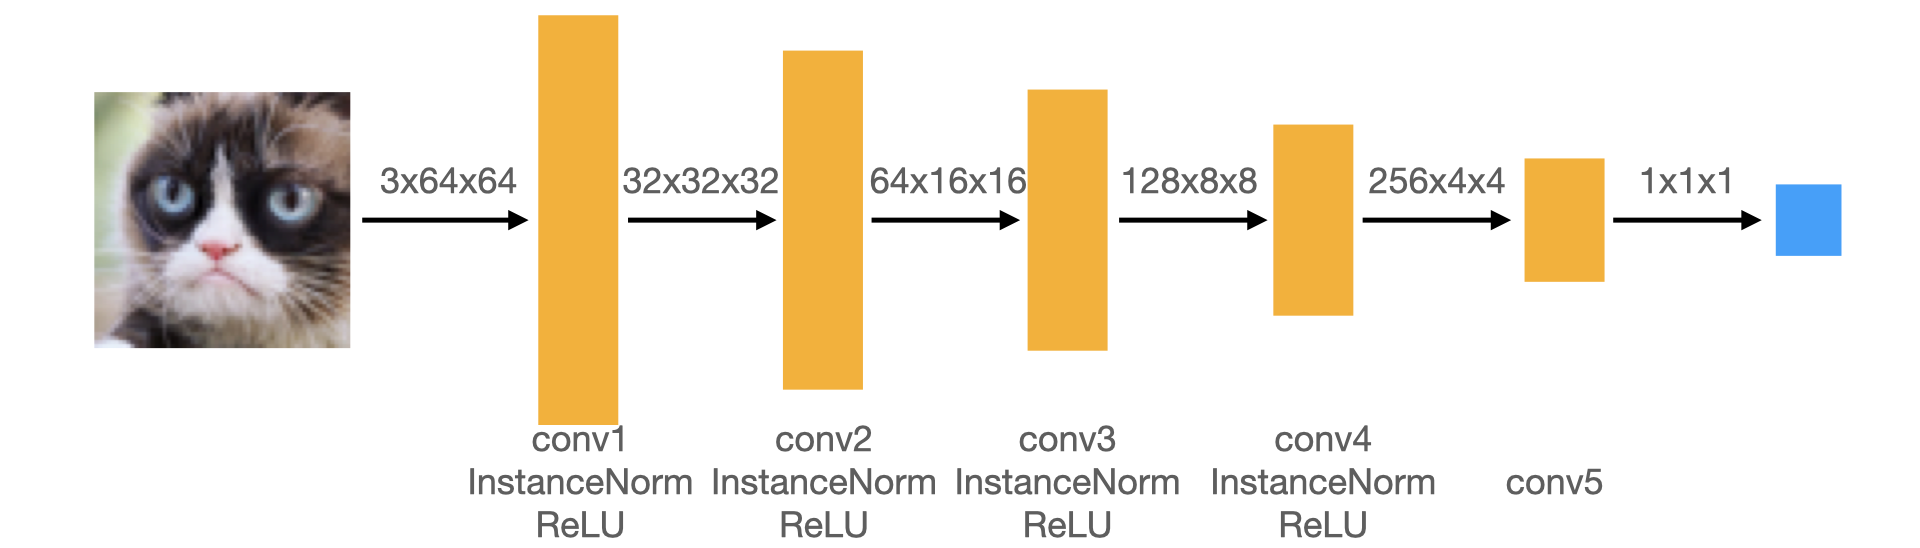
\includegraphics[width=0.9\linewidth]{disc.png}
        % \caption{Enter Caption}
        \label{fig:enter-label}
    \end{figure}
        \begin{itemize}
            \item Padding. In each of the convolutional layers shown above, we downsample the spatial dimension of the input volume by a factor of 2. Given that we use kernel size K = 4 and stride S = 2, what should the padding be? Write your answer on your website, and show your work (e.g., the formula you used to derive the padding).
            \item Implementation. Implement this architecture by filling in the \textbf{\_\_init\_\_} and forward method of the\textbf{ DCDiscriminator} class in \textbf{models.py}, shown below. The\textbf{ conv\_dim} argument does not need to be changed unless you are using larger images, as it should specify the initial image size. Note the function \textbf{conv} is defined in \textbf{models.py}.
        \end{itemize}
    \item Generator. Now, we will implement the generator of the DCGAN, which consists of a sequence of transposed convolutional layers that progressively upsample the input noise sample to generate a fake image. The generator in this DCGAN has the following architecture:
    \begin{figure}[h]
        \centering
        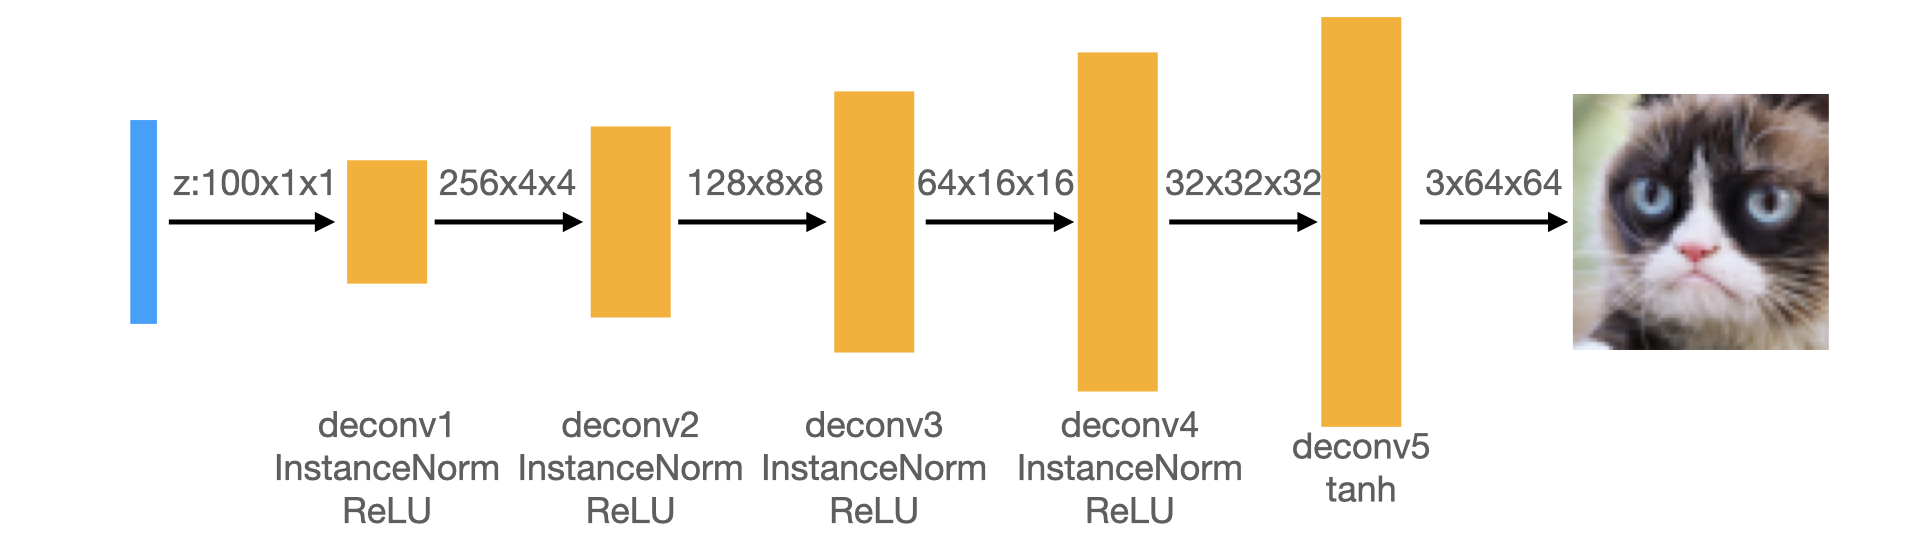
\includegraphics[width=0.9\linewidth]{gene.png}
    \end{figure}
    \begin{itemize}
        \item Implementation. Implement this architecture by filling in the \textbf{\_\_init\_\_} and forward method of the \textbf{DCGenerator} class in \textbf{models.py}. Note: Use the \textbf{deconv} function (analogous to the \textbf{conv} function used for the discriminator above) in your generator implementation.
    \end{itemize}
    \item Training Loop. Next, you will implement the training loop for the DCGAN. A DCGAN is simply a GAN with a specific type of generator and discriminator; thus, we train it in exactly the same way as a standard GAN. The pseudo-code for the training procedure is shown below. The actual implementation is simpler than it may seem from the pseudo-code: this will give you practice in translating math to code. 
    \begin{figure}[h]
        \centering
        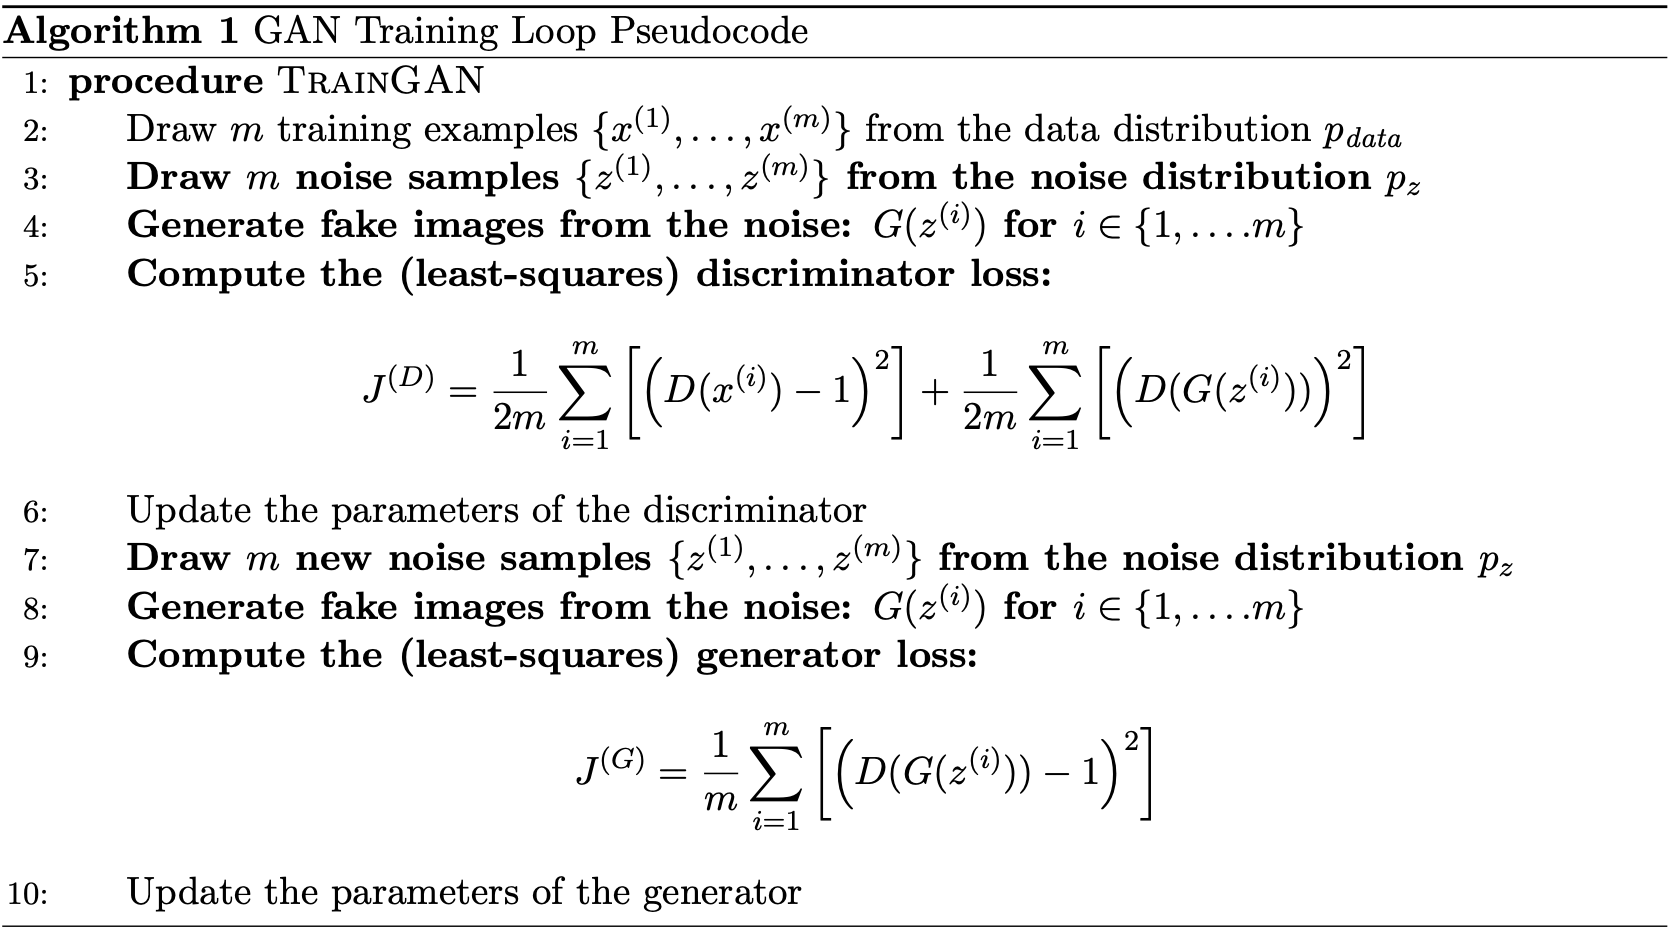
\includegraphics[width=0.9\linewidth]{pseudo.png}
    \end{figure}
    \begin{itemize}
        \item Implementation. Open up the file \textbf{vanilla\_gan.py }and fill in the indicated parts of the \textbf{training\_loop} function. There are 5 numbered bullets in the code to fill in for the discriminator and 3 bullets for the generator. Each of these can be done in a single line of code, although you will not lose marks for using multiple lines.
    \end{itemize}

    \item Experiment. Train the DCGAN with the command:
    \begin{lstlisting}
        python vanilla_gan.py --num_epochs=100
    \end{lstlisting}
    The script saves the output of the generator for a fixed noise sample every 200 iterations throughout training; this allows you to see how the generator improves over time. More command line parameters can be found in \textbf{vanilla\_gan.py}.
    \begin{itemize}
        \item Screenshots of discriminator and generator training loss with both \textbf{data\_aug=basic/deluxe} – 4 curves in total. Briefly explain what the curves should look like if GAN manages to train.
        \item Set data augmentation to deluxe and then show one of the samples from early in training (e.g., iteration 200) and one of the samples from later in training, and give the iteration number for those samples. Briefly comment on the quality of the samples, and in what way they improve through training. (It typically requires more than 3,000 iterations to attain a visually appealing effect. Pictures in the early stages of training will be blurry.)
        
    \end{itemize}
    \item Discussion. 
        \begin{itemize}
            \item DCGAN is more stable than traditional GAN in training, but there are still certain problems. What problems did you find during this training?
            \item How do you think it should be improved? Do other generative models (VAE, Diffusion) also have such problems?
        \end{itemize}
\end{enumerate}


\end{document}
